\section{Architektur}\label{sec:architecture}

Fulib.org verwendet eine einfache Architektur, bestehend aus Frontend, Backend und Datenbank.
Da es sich um eine Webanwendung handelt, wird das Frontend im Browser ausgeführt.
Öffnet man die Seite, werden die benötigten \ac{html}-, JavaScript- und \ac{css}-Dateien vom Backend heruntergeladen und im Browser angezeigt.
Aus Sicht des Backends sind dies statische Ressourcen.
Sämtlicher Datenaustausch in der Webanwendung geschieht dann über \ac{http}-Anfragen an das Backend.
Dabei wird \ac{json} als Datenformat verwendet.
Für die persistente Datenspeicherung von Anfragelogs, Aufgabenblättern, Lösungen, Kursen und Kommentaren kommt eine Mongo-Datenbank~\cite{mongodb} zum Einsatz.
Die Kompilierung und Ausführung von Scenarios wird durch Anbinden des Scenario- und Java-Compilers sowie einer JUnit-Laufzeit bewerkstelligt.
Abbildung~\ref{fig:website-architecture} gibt einen Überblick über die verschiedenen Komponenten, die es der Webseite ermöglichen, ihre Funktionalität bereitzustellen.
Im folgenden Abschnitt wird näher erläutert, wie diese zusammenwirken.

\begin{figure}
    \centering
    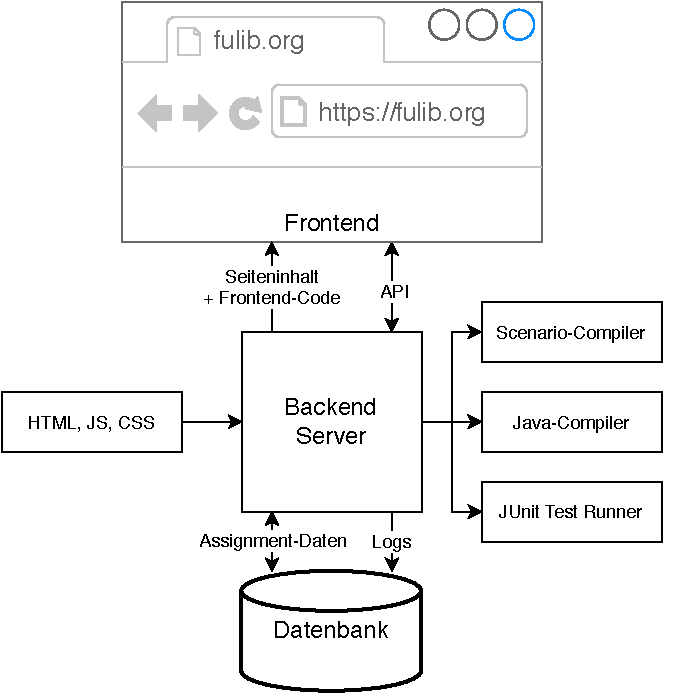
\includegraphics[width=0.5\textwidth]{chapter/fulib.org/img/architecture.pdf}
    \caption{Architektur von fulib.org}
    \label{fig:website-architecture}
\end{figure}

\subsection{Frontend}\label{subsec:frontend}

% Angular
Das Frontend von fulib.org ist mit dem Angular-Framework~\cite{angular} implementiert.
Dieses gibt eine Architektur vor, die Anwendungslogik (Services) von \ac{ui}-Logik (Komponenten) trennt.
Services sind beispielsweise dafür zuständig, mit dem Backend Daten auszutauschen.
Mittels Dependency Injection lassen sich diese von Komponenten oder von anderen Services beziehen.
Die Komponenten befassen sich mit der Darstellung der Anwendung.
Sie bestehen aus einem \ac{html}-Template, eigenem \ac{css} und einer Klasse, die Daten mit Services kommuniziert und die Logik der Benutzeroberfläche implementiert.
Komponenten haben besonders als wiederverwendbare Elemente Bedeutung.
Sie ermöglichen es, gemeinsame Funktionalität zu verkapseln und an mehreren Stellen in der Anwendung zu verwenden.
Im Kontext der Assignments ist beispielsweise die Task-Liste eine Komponente, die auf mehreren Seiten zum Einsatz kommt.
Da Komponenten nur einmal implementiert werden und beliebig oft wiederverwendbar sind, kann die Oberfläche konsistent gehalten und Fehler vermieden werden.

% Bootstrap + Darkmode
Das Aussehen der Oberfläche von fulib.org basiert auf Bootstrap~4~\cite{bootstrap}.
Das \ac{css}-Framework gibt vielen \ac{html}-Elementen wie Buttons oder Eingabefeldern ein modernes Aussehen.
Ferner ermöglicht es die einfache Anordnung von Elementen, die sich an verschiedene Bildschirmgrößen anpassen kann.
Somit ist fulib.org ohne großen Entwicklungsaufwand auch auf Smartphones und anderen Mobilgeräten übersichtlich.
Bei dem im Footer einstellbaren Nachtmodus handelt es sich um Funktionalität, die von der Bootstrap-Darkmode-Bibliothek~\cite{bootstrap-darkmode} bereitgestellt wird.
Diese Eigenentwicklung passt die Farbgebung von Bootstrap so an, dass alle normalerweise weißen oder hellen Elemente in schwarz bzw.\ Grautönen erscheinen.
Dies schont bei dunkleren Lichtbedingungen das Auge.

% CodeMirror
Die Editorfenster für Scenarios und Java-Code sind mit der CodeMirror-Bibliothek~\cite{codemirror} implementiert.
Diese bietet einen Editor, der Syntaxhighlighting für viele Programmier- und Markupsprachen unterstützt.
Der Editor erlaubt die Anpassung der Farbgebung, was auf fulib.org beim Wechsel in den Nachtmodus zu beobachten ist.
Zudem unterstützt der Editor eine Reihe von Addons, die zusätzliche Funktionalität einbringen können.
Beispielsweise ermöglicht ein Lint-Addon die Hervorhebung von Fehlermeldungen im Editor.
Es ist geplant, diese im Scenario-Editor umzusetzen.

\subsection{Backend}\label{subsec:backend}

Beim Backend von fulib.org handelt es sich um einen einfachen \ac{http}-Server.
Dieser ist zustandslos, arbeitet somit nach dem \ac{rest}-Prinzip.
Die Hauptaufgaben des Backends sind die Auslieferung des Frontends, die Ausführung von Scenarios sowie die Kommunikation mit der Datenbank im Kontext von Assignments.

% Frontend
Als Teil des Buildprozesses von fulib.org werden statische \ac{html}-, JavaScript- und \ac{css}-Dateien erzeugt, die das gesamte Frontend umfassen.
Diese werden vom Backend auf Anfrage eines Browsers unverändert an diesen übermittelt.
Anders als bei serverseitig generierten Webseiten hat dies den Vorteil, dass der Ressourcenaufwand des Servers sehr gering ist.
Auch lassen sich die statischen Ressourcen sehr gut zwischenspeichern, beispielsweise in einem Cache oder im Browser.
Dadurch können, mit Ausnahme vom ersten Besuch der Seite, die Ladezeiten erheblich verkürzt werden.
Der Aufwand steigt jedoch auf Client- bzw.\ Browserseite, der nach Herunterladen der statischen Dateien das JavaScript ausführen muss, um den Webseiteninhalt aufzubauen.
Dieser Vorgang kann bei weniger leistungsfähigen Geräten für längere Verzögerungen sorgen.
Ebenso ist zu beachten, dass fulib.org bei deaktiviertem oder nicht unterstützem JavaScript zwar aufrufbar, jedoch nicht verwendbar ist.
In diesem Fall wird eine Meldung in Form eines Banners angezeigt, die den Benutzer zur Aktivierung auffordert und dafür Hilfe anbietet.

% Scenario Compile and Run
Die Ausführung der Scenarios delegiert das Backend an die drei zuständigen Tools.
Nacheinander werden Scenario- und Java-Compiler sowie der JUnit-Testprozess ausgeführt.
Der Server schreibt zunächst den über die \ac{api} empfangenen Text in eine Datei in einem temporären Ordner.
Daraufhin wird der Scenario-Compiler in diesem Ordner ausgeführt, der die Java-Dateien sowie das Klassendiagramm generiert.
Mit dem Java Compiler wird der Java-Code dann kompiliert und die entstehenden Klassen dynamisch geladen.
Das JUnit-Framework bietet eine Schnittstelle zum Ausführen der Test-Klassen an, wodurch das Testergebnis sowie die Objektdiagramme entstehen.
Die Ausgaben der drei Tools werden dabei protokolliert, da diese Teil der Antwort werden.
Der temporäre Ordner wird anschließend nach Diagramm- und Java-Dateien durchsucht.
Diagramme werden unter Anwendung einer geeigneten Codierung in die \ac{api}-Antwort übernommen.
Aus Java-Dateien werden relevante Methodenrümpfe durch einen einfachen Parser extrahiert.

% Database
Die Kommunikation mit der Datenbank ist besonders bei Assignments und verwandter Funktionalität relevant.
Alle dafür zuständigen Endpunkte lesen entweder aus der Datenbank oder erzeugen darin neue Datensätze.
Beim Anlegen ist das Anfrageformat stets \ac{json}, das der Server zunächst in sein eigenes Datenmodell konvertiert.
Dieses wird beim Speichern in der Datenbank in deren natives Format konvertiert.
Umgekehrt ist es bei Leseanfragen, bei denen der Server Anfragen an die Datenbank stellt, deren Ergebnis in sein Datenmodell konvertiert und dies als \ac{json} in der Antwort zurückgibt.
Das Backend ist bei sämtlichen Anfragen für die Prüfung von Tokens zur Autorisierung zuständig, wobei sichergestellt wird, dass keine Daten bei unbefugten Anfragen preisgegeben werden.
Diese Prüfung wird insbesondere nicht im Frontend durchgeführt, da sonst ein Angreifer manuell die Server-\ac{api} ansprechen und ausnutzen könnte.
